\documentclass[twoside]{article}

\usepackage[math]{kurier}
\usepackage[sc]{mathpazo}                 
\usepackage{amsmath}
\usepackage{graphicx}
\renewcommand{\sfdefault}{kurier}


\usepackage{graphics}
\setlength{\oddsidemargin}{0.25 in}
\setlength{\evensidemargin}{-0.25 in}
\setlength{\topmargin}{-0.6 in}
\setlength{\textwidth}{6.5 in}
\setlength{\textheight}{8.5 in}
\setlength{\headsep}{0.75 in}
\setlength{\parindent}{0 in}
\setlength{\parskip}{0.1 in}


\newcounter{lecnum}
\renewcommand{\thepage}{\thelecnum-\arabic{page}}
\renewcommand{\thesection}{\thelecnum.\arabic{section}}
\renewcommand{\theequation}{\thelecnum.\arabic{equation}}
\renewcommand{\thefigure}{\thelecnum.\arabic{figure}}
\renewcommand{\thetable}{\thelecnum.\arabic{table}}


\newcommand{\lecture}[4]{
   \pagestyle{myheadings}
   \thispagestyle{plain}
   \newpage
   \setcounter{lecnum}{#1}
   \setcounter{page}{1}
   \noindent
   \begin{center}
   \framebox{
      \vbox{\vspace{2mm}
    \hbox to 6.28in { {\bf \sffamily AA 274: Principles of Robotic Autonomy
                        \hfill Winter 2018} }
       \vspace{4mm}
       \hbox to 6.28in { {\sffamily{\Large \hfill Lecture #1: #2  \hfill}} }
       \vspace{2mm}
       \hbox to 6.28in { {\it \hfill Scribes: #4} }
      \vspace{2mm}}
   }
   \end{center}
   \markboth{Lecture #1: #2}{Lecture #1: #2}

   \vspace*{4mm}
}



%%%%%%%%%%%%%%%%%%%%%%%%%%
%document
\begin{document}
%modify this
\lecture{6}{Stereo Vision and Structure from Motion}{}{Gael Gurvan Colas, Soyeon Jung, Greg Katz}

\section{Introduction}

	This lecture \cite{slides} covers geometric concepts needed for 3D reconstruction.  The common methods for reconstructing a 3D scene from 2D images are :
\begin{enumerate}
\item Recognition of landmarks
\item Depth from focus
\item Stereo vision
\item Structure from motion. 
\end{enumerate}

	Recognition of landmarks utilizes known characteristics of particular structures such as orthogonal walls. Depth from focus determines distance to a point by taking multiple images with progressively better focus. Stereo vision triangulates the distance of a point in 3D by its coordinates in two distinct images taken at the same time by cameras with known relative pose. Structure from motion processes multiple images taken at different times. A key aspect of stereo vision and structure from motion is finding point correspondences across multiple images. Much of this lecture covers geometric constraints used to narrow the search space for finding point correspondences. Complementary readings \cite{SNS, FP}

\section{Method \#1 Depth from Focus}

\begin{figure}[h!]
  \begin{center}
    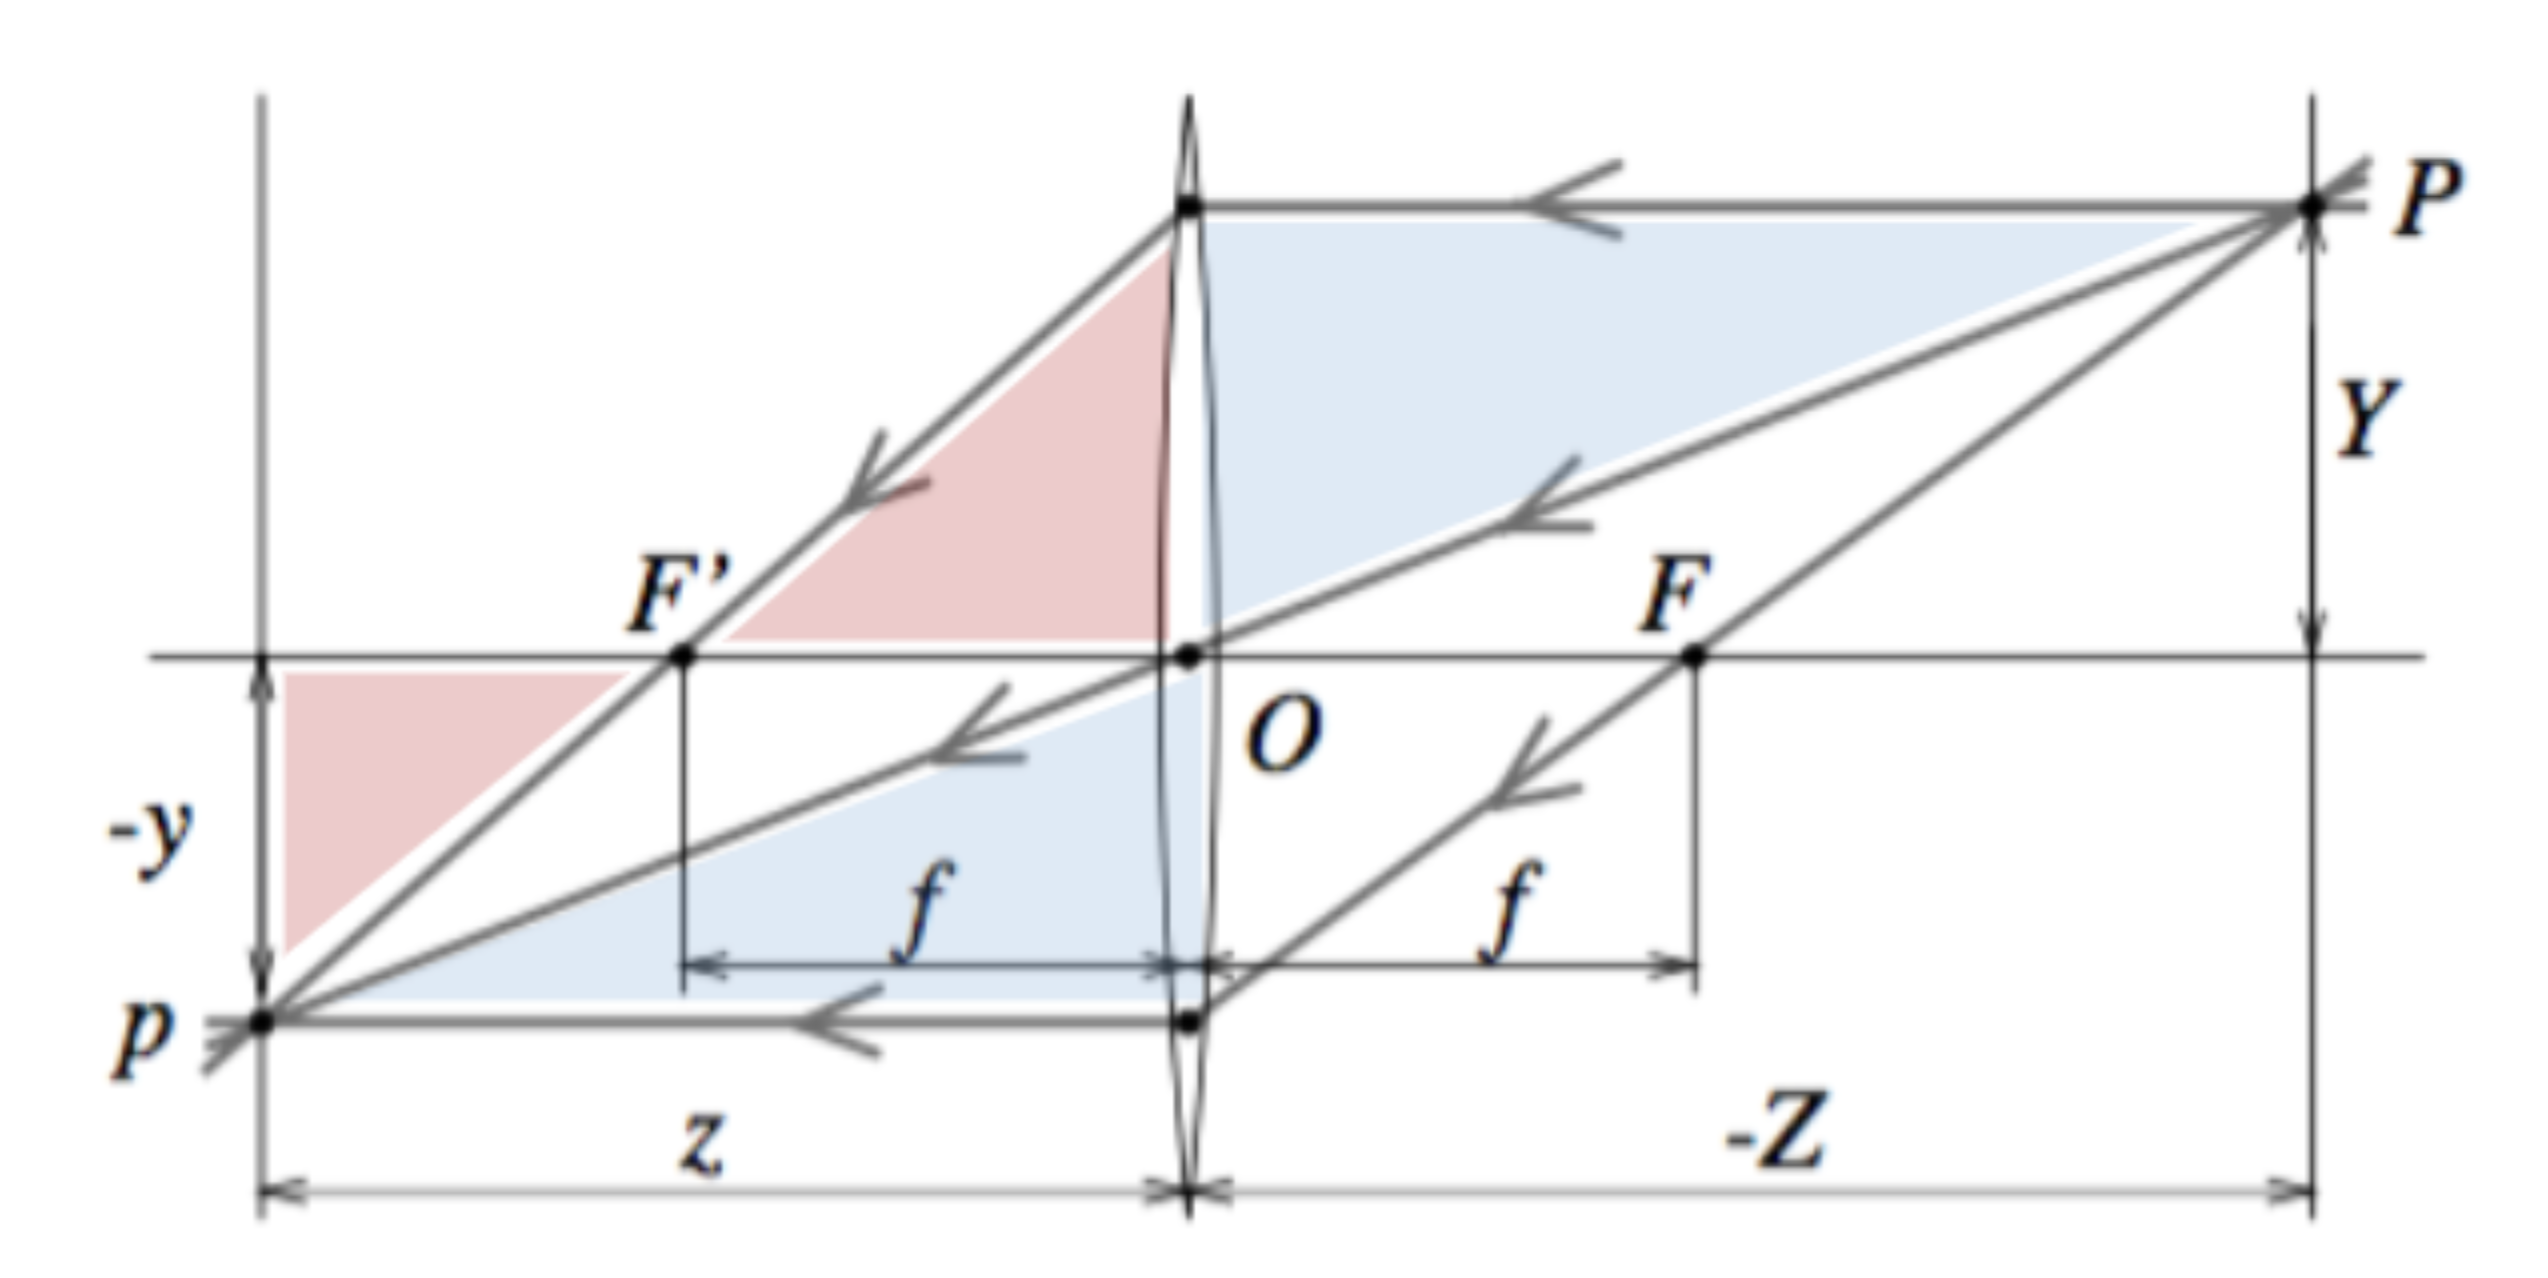
\includegraphics[scale=0.2]{thinlens}
  \end{center}
  \caption{Projection of a point through a thin lens}
  \label{lens}
\end{figure}

An ideal thin lens (Figure \ref{lens}) focuses rays of light emitting from a point $P$ at a depth $Z$ from the center of the lens to a point $p$ at a distance $z$ from the center of the lens. The distance $z$ is called the focal distance. By properties of similar triangles it can be shown that such points must obey the thin lens constraint (Equation \ref{tlc}).
\begin{align}
  \label{tlc}
  \frac{1}{z} + \frac{1}{Z} = \frac{1}{f}
\end{align}

Thus if the focus distance $z$ and focal length $f$ are known, the depth, $Z$ of the point $P$ can be obtained. We assume the focal length is known as a property of the lens. The focus distance $z$ is found by trying different values until the projection of the point in question becomes sharp in the image. 

In practice this technique is not often used because different focus distances must be found for every point in the image which is not at the same depth. 

\section{Method \#2 Stereopsis}

In practice, a more powerful technique used to reconstruct 3D scenes from 2D images is the process of fusing two images into one, known as stereopsis. This is how humans see. And indeed it has been demonstrated to be effective in robotics, this is on what the vision of Mars rovers is based.

In principle, the depth of $P$ can be obtained from the intersection of two lines of sight (Figure \ref{triangle}). In other words, given $\overline{Op}$ and $\overline{O'p'}$ the point $P$ is determined by the intersection of these lines and this process is called triangulation. To know $\overline{Op}$ and $\overline{O'p'}$ in a  world coordinate frame fixed for one of the cameras, the relative pose of the cameras and their intrinsic matrices must be known.

\begin{figure}[h!]
  \begin{center}
	\begin{tabular}{cc}
	  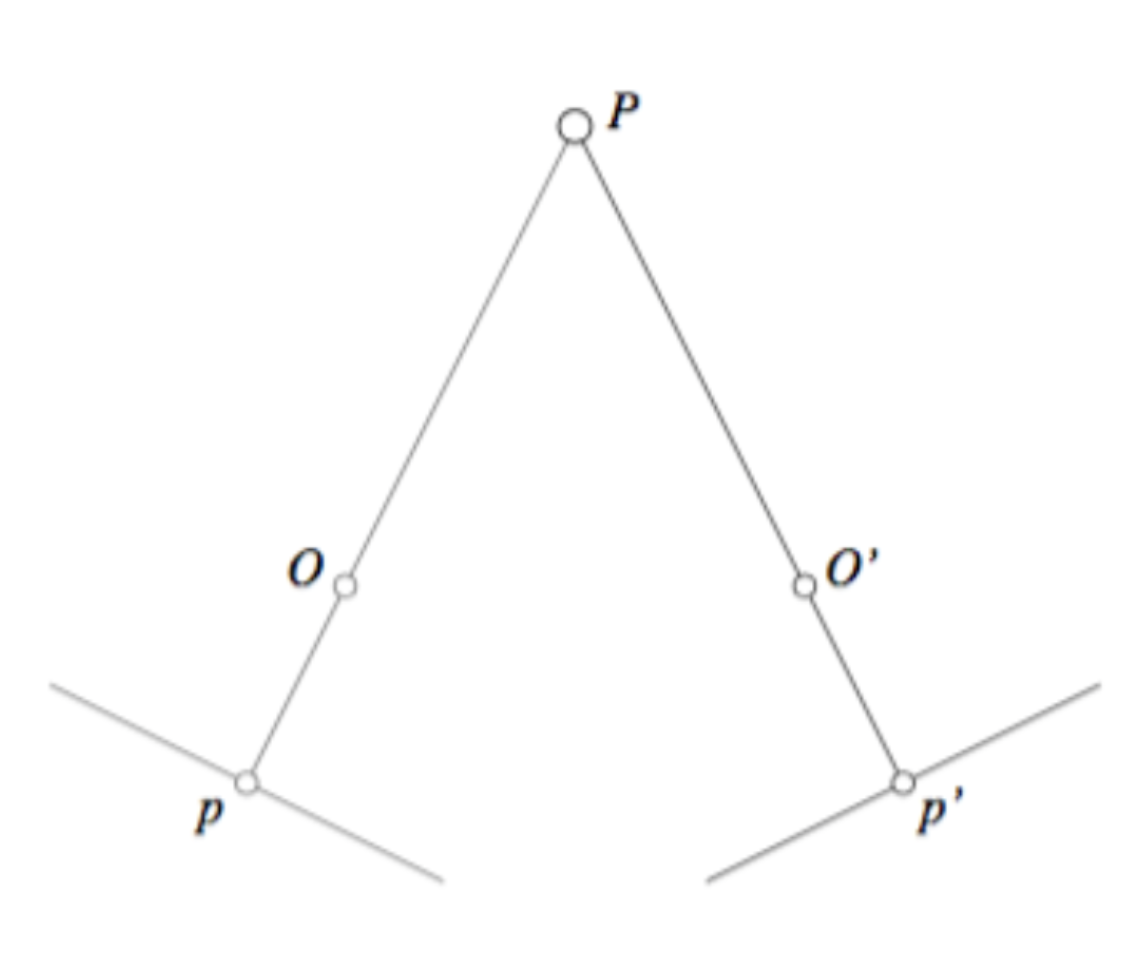
\includegraphics[scale=0.3]{triangulation.png}
	  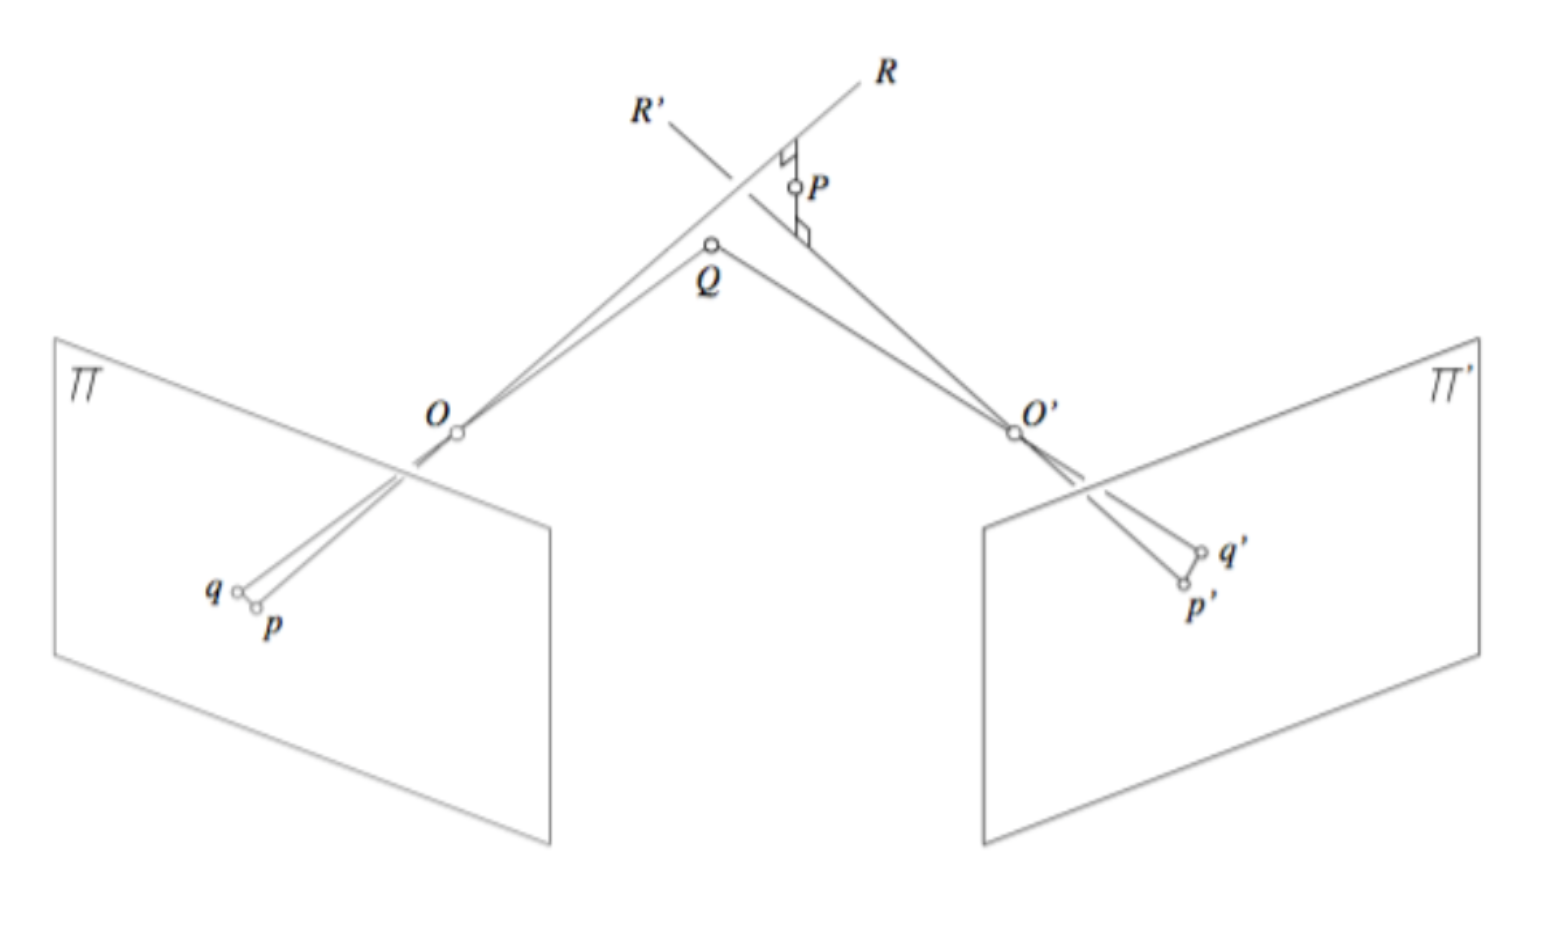
\includegraphics[scale=0.3]{approximation.png}
	\end{tabular}
  \end{center}
  \caption{The triangulation principle in 2D (left), the approximation in 3D (right)}
  \label{triangle}
\end{figure}

Due to noise in the measurement and calibration it is essentially impossible for the two lines of sight to precisely intersect in 3D (Figure \ref{triangle}). Since there is no single point that can exactly correspond to the observations, in practice, $P$ is approximated by finding the 3D-point $Q$ that best explains the observations. I.e. the point whose projection in the two image planes is closest to the observed points. This is computed in term of the following metric known as the re-projection error :
\begin{align}
Q = \arg\!\min_Q (d^2(p, q) + d^2(p', q'))
\end{align}

where $q$ and $q'$ are the projection of $Q$ onto the two camera images planes and $p$ and $p'$ are observed point correspondences in the image planes.

\subsection{Stereo vision process}

So far we have seen that given corresponding projected points in two images from a calibrated camera, we can reconstruct the coordinates of the original point in 3D. This is actually the second step of the two-step stereo vision process : 

\begin{enumerate}
  \item Correspondence: fusion of features observed by two (or more) cameras
  \item Triangulation: reconstruction of three-dimensional pre-images
\end{enumerate}

The first step is finding corresponding points in the two images. In practice this is the more challenging step of the two. In the general case, finding correspondences requires a search in two dimensions between all points in each image, but several constraints can be leveraged to restrict this search, such as similarity constraints, continuity constraints, and most importantly the \emph{epipolar} constraint. 

The epipolar constraint intrinsically specifies the geometry of stereo vision. Specifically, given a point in one image the epipolar constraint limits the location of the corresponding point in the other image to a line, thus reducing the search space for correspondence from two dimensions to one. 

\subsection{Epipolar geometry}

Consider the following problem: we know the relative positions and orientations of two calibrated cameras. We have an observation of a point $p$ in our first image plane and we want to find a constraint that helps in finding the corresponding point $p'$ in the second image plane, where $p$ and $p'$ are projections of the same point $P$ in the 3D.

We start by defining the \emph{epipolar plane} as the plane that passes through $O$, $O'$, and $p$. Since $p$ and $p'$ are on the lines $\overline{OP}$ and $\overline{O'P}$, we know that $P$ and $p'$ also lie on the epipolar plane. Now consider virtual image planes $\Pi$ and $\Pi'$ in front the camera centers. These planes are known since we assumed our cameras are calibrated. Since $p'$ must lie both on the epipolar plane and the virtual plane $\Pi'$, then $p'$ must lie on the intersection of the epipolar plane and the virtual image plane. This intersection line is called the \emph{epipolar line}. Thus, given $O$, $O'$, $p$, and the image plane $\Pi'$ we have constrained the location of the corresponding point $p'$ to a line in $\Pi'$. 

In the figure \ref{epi}, note that $O$, $O'$, and $p$ are known. $P$ is not known precisely, but we must be somewhere along $\overline{Op}$. Then, the line of sight from the second camera to $P$ must pass through $O'$ and the line $\overline{Op}$. These candidate lines are red in figure \ref{epi}. These candidate lines cross the image plane $\Pi'$ at points that form the epipolar line. 

\begin{figure}[h!]
  \begin{center}
	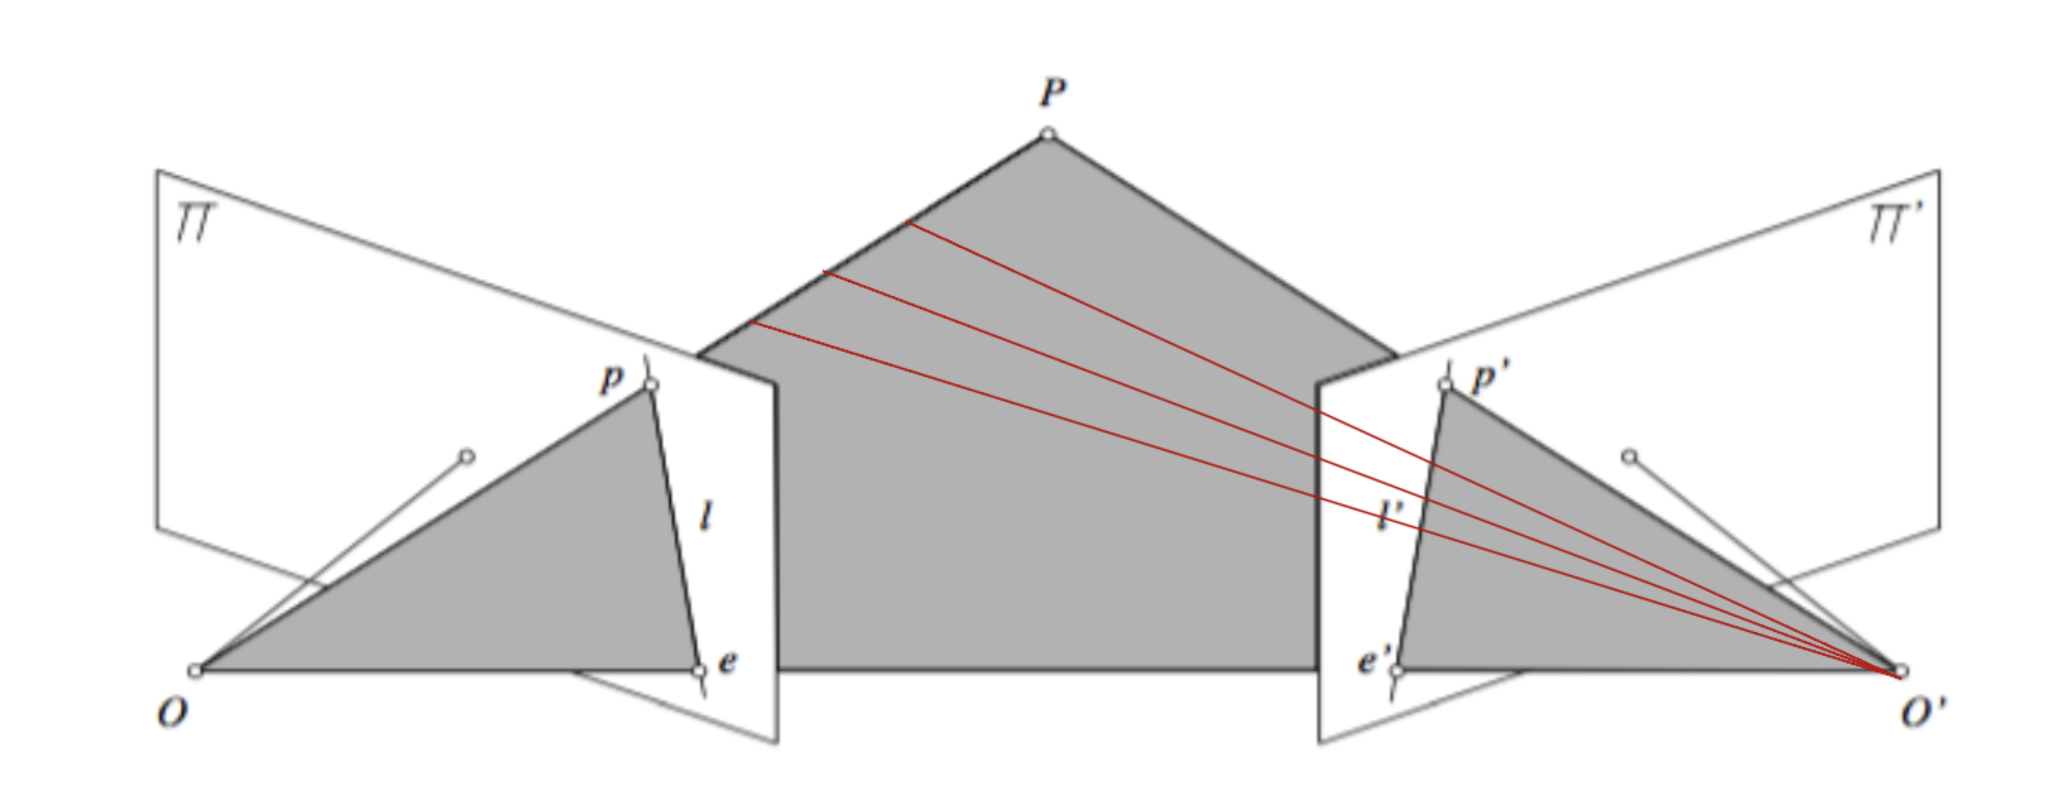
\includegraphics[scale=0.3]{epipolar.png}
  \end{center}
  \caption{The epipolar plane}
  \label{epi}
\end{figure}

Summary of terminology:
\begin{itemize}
\item \textbf{Epipolar plane}: The plane containing the points O, O', p, p', and P
\item \textbf{Baseline}: the line connecting the centers, $\overline{OO'}$
\item \textbf{Epipolar lines}: The intersection of the epipolar plane and the image planes, respectively $l$ and $l'$
\item \textbf{Epipoles}: the intersection points of the baseline and the virtual image planes, respectively $e$ and $e'$
\item \textbf{Epipolar constraint}: potential correspondences for $p$ must lie on the epipolar line $l'$ (and vice versa)
\end{itemize}

Figure \ref{correspondence} shows an example of corresponding points from two images and the epipolar line. 

\begin{figure}[h!]
  \begin{center}
	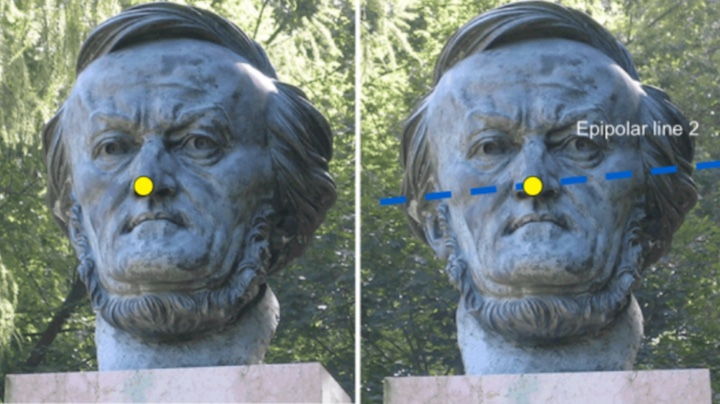
\includegraphics[scale=0.3]{correspondence2.jpg}  \end{center}
  \caption{An example of computed epipolar plane (left) from a initial point (right)}
  \label{correspondence}
\end{figure}

\subsubsection{Epipolar geometry and the Essential Matrix}

To define the epipolar constraint mathematically, we use the fact that $\overline{Op}$, $\overline{O'p'}$, and $\overline{OO'}$ are coplanar to write:

\begin{align}
\overline{Op} \cdot [\overline{OO'} \times \overline{O'p'}] = 0.
\end{align}

To see this is true, note that $\overline{OO'} \times \overline{O'p'}$ is a vector perpendicular to the epipolar plane, and consequently perpendicular to $\overline{Op}$. The dot product of these perpendicular vectors is then defined to be 0. 

Now assume that the world reference system is co-located with camera 1. Define normalized coordinates $\hat{p} = K^{-1}p$ and $\hat{p'} = K'^{-1}p'$. Define the rotation matrix between camera 1 and camera 2 as $R$ so in the camera 1 reference frame $\overline{O\hat{p'}} = R\hat{p'}$. Define the translation from camera 1 to camera 2 as $t$ so $\overline{OO'} = t$. Then our coplanar constrain becomes

\begin{align}
\hat{p} \cdot [t \times (R\hat{p'})] = 0.
\end{align}

Note that a cross product can be expressed as the product of skew-symmetric matrix and a vector.

\begin{align}
a \times b &= [a]_x b \\
\text{where } [a]_x &= \begin{bmatrix}
0 & -a_3 & a_2 \\
a_3 & 0 & -a_1 \\
-a_2 & a_1 & 0 
\end{bmatrix} .
\end{align}

Then the epipolar constraint can be written as a product of matrices as :
\begin{align}
\hat{p} \cdot [t \times (R\hat{p'})] &= \hat{p} [t]_x R \hat{p'} = \hat{p}E\hat{p'} = 0. \\
\text{where } E &= [t]_xR.
\end{align}

We now have a single matrix that defines the epipolar constraint for any normalized point correspondences between two calibrated cameras. If we note that a line in homogeneous coordinates is defined by the points that satisfy $p \cdot l = 0$ then we can see right away that the epipolar lines can be calculated as:
\begin{align}
l &= E\hat{p'} \\
l' &= E^T\hat{p}.
\end{align}

For the special case of the epipoles the epipolar line is undefined because $t$ and the epipoles are parallel so $E^Te = Ee' = 0$. This leads to the resul that $E$ is singular (non-invertible). Finally, we make note that $E$ has five degrees of freedom - 3 for $R$ and 2 for $t$ due to scaling ambiguity.

\subsubsection{Epipolar geometry and the Fundamental Matrix \cite{FP}}

To generalize the essential coordinates to native coordinate (as opposed to normalized coordinates) we note that $p = K\hat{p}$ and $p' = K'\hat{p'}$. The epipolar constraint then becomes

\begin{align}
p^TK^{-T}EK'^{-1}p' &= p^T F p' = 0 \\
\text{where } F &= K^{-T}E K'^{-1} = K^{-T}[t]_x R K'^{-1}.
\end{align}

Once again we have epipolar lines as 
\begin{align}
l &= Fp' \\
l' &= F^Tp.
\end{align}

$F$ is also singular because $F^Te = Fe' = 0$. Finally $F$ is defined by 9 elements but is constrained by det(F) = 0 and a common scaling so in the end $F$ has only 7 degrees of freedom.

\subsubsection{Computing the Fundamental Matrix}

Given the fundamental matrix $F$, we can compute a specific epipolar line in image 2 that corresponds to a point $P$ in image 1 without any additional information, as shown in Figure \ref{ex2}

\begin{figure}[h!]
  \begin{center}
	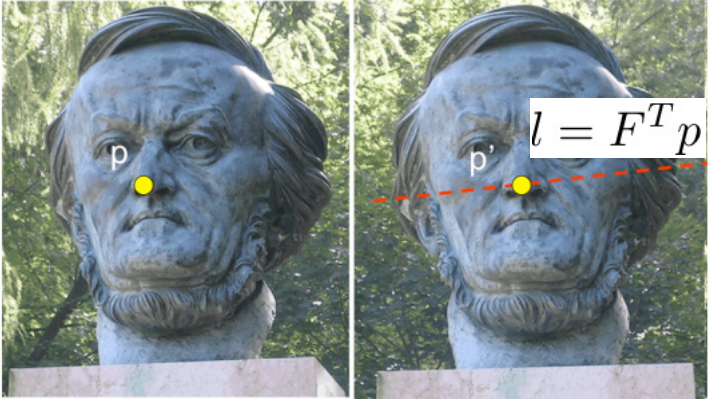
\includegraphics[scale=0.45]{correspondence3.PNG}  \end{center}
  \caption{An example of computed epipolar line and point $p'$ that correspond to a point $p$ (left)}
  \label{ex2}
\end{figure}

To compute a fundamental matrix, we use the same approach as we did for projection matrix. We find a number of correspondences, for example by Brute Force search, using clearly distinguishable points such as corners. 

Assume we are given a number of corresponding points $p = [u, v, 1]^T$ and $p'= [u',v',1]^T$ expressed in a homogeneous coordinate. Each pair of points has to satisfy the epipolar constraint $F$.

\begin{align}
[u, v, 1] \begin{bmatrix}
F_{11} & F_{12} & F_{13} \\
F_{21} & F_{22} & F_{23} \\
F_{31} & F_{32} & F_{33} 
\end{bmatrix} \begin{bmatrix}
u' \\ v' \\ 1
\end{bmatrix} &= 0
\end{align}

We can rewrite this into a scalar product of two one-dimensional vectors. The first vector contains the known coefficients from the given points and the second vector contains each element of the fundamental matrix. Now we have a scalar euqation, therefore one constraint, for each pair of given points.

\begin{align}
[uu', uv', u, vu', vv', v, u', v', 1]\begin{bmatrix}
F_{11} \\F_{12} \\F_{13} \\F_{21} \\F_{22} \\F_{23} \\F_{31} \\F_{32} \\F_{33}
\end{bmatrix} = Wf = 0
\end{align}

As in the projection matrix, the fundamental matrix can be defined up to scale, e.g. normalized by the last component. Therefore, we need 8 parameters to estimate 9 entries of the fundamental matrix. Given $n>=8$ correspondences, we can solve $\tilde{F}$

\begin{align}
\min_{f\in{R^9}}\|Wf\|^2 \\
\text{subject to } \|f\|^2 = 1
\end{align}

Here, while $\tilde{F}$ satisfies the epipolar constraints, it is not necessarily singular. we can enforce rank-2 constraint via SVD decomposition to get the proper fundamental matrix from the candidates.

\begin{align}
\arg\!\min_F \|F-\tilde{F}\|^2 \\
\text{subject to } det(F) = 0
\end{align}

\subsubsection{Image Rectification}

Assume we have two parallel image planes. Now, the epipolar lines are horizontal and $v$ coordinates are equal, both triangulation and correspondence can be done much simpler. We can warp images to simulate a parallel image plane through a process called "Image Rectification" (Figure \ref{rect}). This process exploits some algorithms applying projective transformation, which will not be discussed in this lecture. So let's assume we have rectified image pairs.

\begin{figure}[h!]
  \begin{center}
	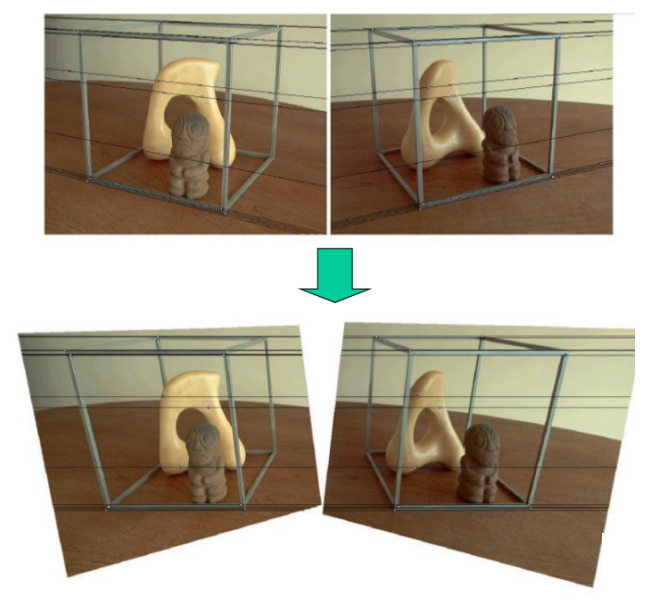
\includegraphics[scale=0.5]{rectified_image.PNG}  \end{center}
  \caption{Image Rectification}
  \label{rect}
\end{figure}

Recall that stereo vision consists of two steps: correspondence and triangulation. This lecture will focus on the triangulation problem. A preimage point $P$ is projected on two image planes to be $p_u$ and $p'_u$. $u$ is the horizontal coordinate and $v$ is the vertical coordinate. Because the epipolar line is horizontal, $p_u$ and $p'_u$ have the same vertical coordinate, and we do not consider $v$ coordinates.

Knowing the horizontal projection of $p$ into two cameras, we can estimate the distance $z$ of the point from the similar triangles (Figure \ref{recttri}).

\begin{align}
%   \label{tlc}
  \frac{z}{b} &= \frac{z-f}{b-p_u+p'_u} \\
  \ z &= \frac{bf}{p_u-p'_u}
\end{align}

\begin{figure}[h!]
  \begin{center}
	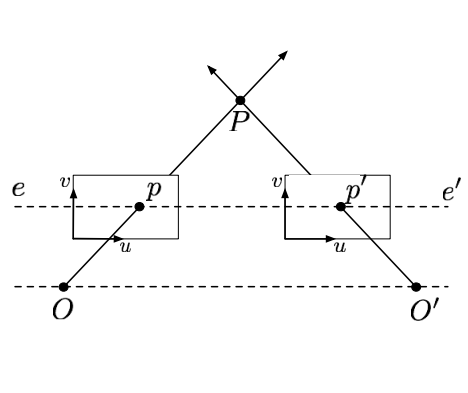
\includegraphics[scale=0.45]{rectified_triangulation_1_.PNG}
	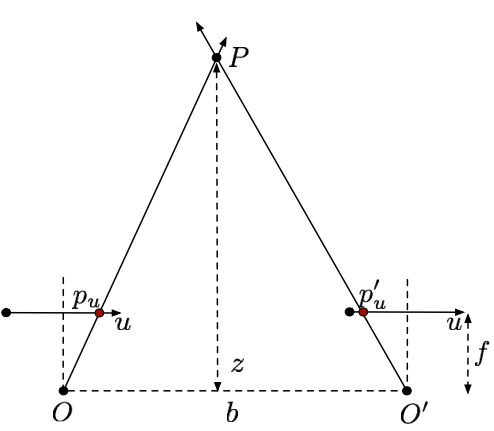
\includegraphics[scale=0.4]{rectified_triangulation_2_.PNG}  \end{center}
  \caption{Triangulation under Rectified Images (horizontal view on the left, top-down view on the right)}
  \label{recttri}
\end{figure}

Here $b$ is the baseline and $f$ is the focal length. If the baseline is very large, we have more resolution to estimate the distance $z$, some points may only be visible from one camera. If the baseline is small, we do not have problems in correspondences, we will have a larger relative error in the estimation of $z$.

We can measure the distance by knowing the disparity $p_u-p'_u$, ie the pixel displacement between corresponding points. From the 2 images, we can build a disparity map, an image that plots the disparity values for every pixel from two stereo images (See Fig. 6.8.) Brighter color indicates larger disparities, which means the point is closer to the camera.

\begin{figure}[h!]
  \begin{center}
	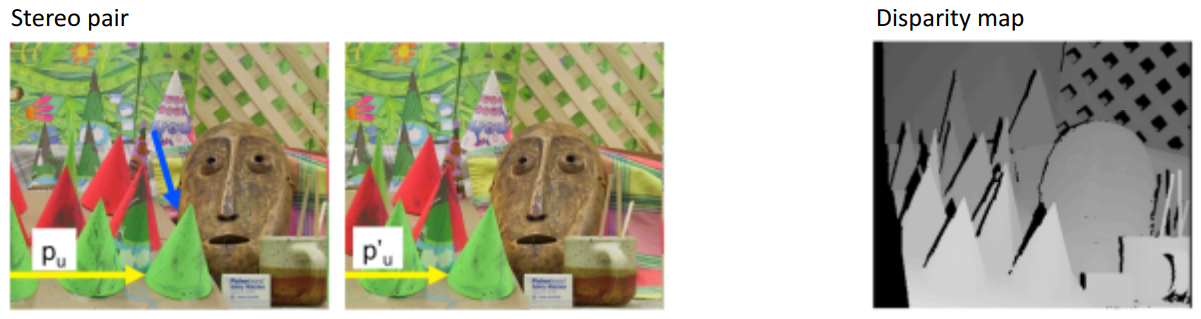
\includegraphics[scale=0.5]{disparity_map.PNG}  \end{center}
  \caption{Disparity Map from a pair of Stereo Images} 
  \label{ex}
\end{figure}

\newpage
\section{Method \#3 Structure From Motion (SFM)}

The Structure From Motion (SFM) method uses a similar principle than Stereopsis but in a different fashion : we do not take images from two cameras at the same time, but instead we take images from one camera at different points in time as we move the camera around the object. Here, the intrinsics parameters are the same because we are using one camera, but the extrinsic changes as we move the camera.

\begin{figure}[h!]
  \begin{center}
	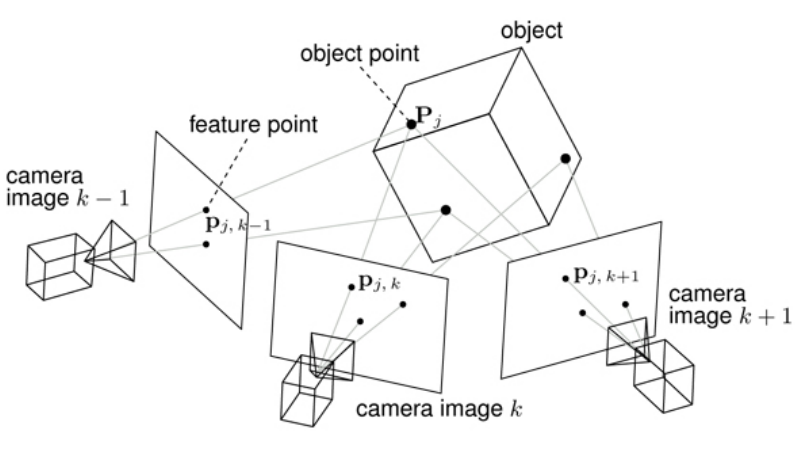
\includegraphics[scale=0.4]{SFM.PNG}  \end{center}
  \caption{Structure From Motion (SFM)} 
  \label{ex}
\end{figure}

Let's consider we have different points $P_j$ on an object and we take the image at time $k$. Given $m$ images of $n$ fixed 3D points, we get $m$ projection matrices $M_k$ (for the $k$th image) : $p_{j,k}^h = M_k P_j^h$.
Where $p_{j,k}$ is the projection of the point $P_j$ on the camera image $k$.

However, SFM is difficult to use because it has ambiguities. That is, we cannot recover the absolute scale of the observed scene. If we have a bigger object in a longer distance in one situation and a smaller object in a closer distance, the projections will be the same (see Figure \ref{amb}). To address this ambiguity, we can take several approaches such as algebraic approach (by fundamental matrix) and bundle adjustment. 

\begin{figure}[h!]
  \begin{center}
	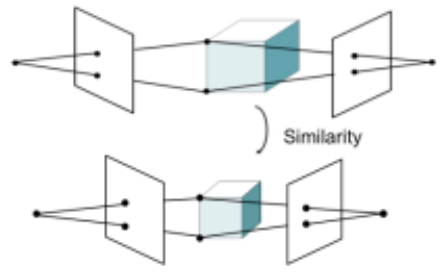
\includegraphics[scale=0.8]{SFM_ambiguities.png}  
  \end{center}
  \caption{Ambiguity in the projection of an object using SFM} 
  \label{amb}
\end{figure}

The concept of SFM is similar to visual odometry, which estimate the motion of a robot by using visual inputs in series. This is widely used in reality, including on Mars by rovers. SFM can be a very powerful method because it not only allows us to reconstruct the environment but also to recover the motion of the camera.

\newpage

\bibliographystyle{unsrt}
\bibliography{references}

\end{document}









